\documentclass[../main/main.tex]{subfiles}

\newdate{date}{13}{12}{2019}


\begin{document}


\subsection{Solution of \eqref{eq:17_13} by Fourier transform}
\marginpar{ \textbf{Lecture 18.} \\  \displaydate{date}. \\ Compiled:  \today.}
Let us  do the Fourier transform of Eq.\eqref{eq:17_13}:
\begin{equation*}
  \qty(- \grad ^2 + \xi ^{-2} (t)) G_c (\va{r}-\va{r}') = \frac{k_B T}{k} \delta (\va{r}-\va{r}')
\end{equation*}
If we define \( \va{x} \equiv \va{r} - \va{r}' \) and we use the following convention for the Fourier transform \( \widetilde{G} (q)  \) of \( G \):
\begin{equation*}
  \widetilde{G} (q) = \int_{- \infty }^{+ \infty }  G_c ( \abs{\va{x}} ) e^{- i \va{q} \vdot \abs{\va{x}} } \dd[d]{\abs{\va{x}} }
\end{equation*}
then transforming both sides of the equation we get:
\begin{equation}
  \qty(q^2 + \xi ^{-2}) \widetilde{G} ( q ) = \frac{k_B T}{k} \quad
   \Rightarrow \widetilde{G} ( q ) = \frac{k_B T}{k} \frac{1}{q^2 + \xi ^{-2}}
\end{equation}
where \( q = \abs{\va{q}}  \).
From this last equation we can also see that when \( T=T_c \), since \( \xi \rightarrow \infty  \)  we have \( \widetilde{G} (q) \simeq \frac{1}{q^2}  \) and so performing the inverse Fourier transform one gets
\begin{equation*}
  G_c (\abs{\va{x}} ) = \abs{\va{x}}^{2-d}
\end{equation*}
from which we have that the critical exponent \( \eta  \)  is null (we will see that explicitly once we have computed \( G \)). In fact, at \( T=T_c \) we have previously defined
\begin{equation*}
  G (r) \sim \abs{\va{x}}^{2-d- \eta }
\end{equation*}
hence, in this case we have \( \eta =0 \).
 Therefore, reminding that  \( \va{x} \equiv \va{r} - \va{r}' \) we can now determine \( G (\va{x}) \)  with the Fourier antitransform:
\begin{equation}
  G (\va{x}) = \int_{}^{}   \frac{\dd[d]{\va{q}}}{(2 \pi )^d} \frac{e^{i \va{q} \vdot \va{x}} }{q^2 + \xi ^{-2}}
\end{equation}
This integral is a bit tedious to compute, and in general its result depends strongly on the dimensionality \( d \) of the system; the general approach used to solve it is to shift to spherical coordinates in \( \R^d \) and then complex integration for the remaining part, which involves \( \abs{\va{q}}  \). In order to do some explicit computations, let us consider the case \( d=3 \); we will then have:

\begin{equation*}
\begin{split}
G(\va{x}) & =   \int_{}^{}  \frac{ \dd[3]{\va{q}}}{(2 \pi )^3} \frac{e^{i \va{q} \vdot \va{x}}}{q^2 + \xi ^{-2}}  \overset{\substack{ \text{spherical} \\ \text{coordinates}} }{=}
= \frac{1}{ (2 \pi )^3} \int_{0}^{\infty }  \frac{q^2}{q^2+ \xi ^{-2}} \dd[]{q} \int_{-1}^{+1}    e^{i q \abs{\va{x}} \cos \theta  } \dd[]{(\cos \theta  )} \int_{0}^{2 \pi } \dd[]{ \varphi}
\\
 &\overset{z \equiv \cos(\theta ) }{=}  \frac{2 \pi }{(2 \pi )^3} \int_{0}^{\infty }  \frac{q^2}{q^2 + \xi ^{-2}} \dd[]{q} \qty[\frac{  e^{i q \abs{\va{x}} z } }{i q \abs{\va{x}} } ]_{-1}^{1}
 = \frac{1}{(2 \pi )^2 \abs{\va{x}} } \int_{0}^{\infty } \frac{q \sin(q \abs{\va{x}} ) }{q^2 + \xi ^{-2}} \dd[]{q}
\end{split}
\end{equation*}
This last integral can be computed, using the residue theorem, extending it to the complex plane:
\begin{equation*}
  I = \int_{0}^{\infty } \frac{q \sin(q \abs{\va{x}} ) }{q^2 + \xi ^{-2}} \dd[]{q}
  = \frac{1}{2} \int_{- \infty }^{+ \infty } \frac{q \sin(q \abs{\va{x}} ) }{q^2 + \xi ^{-2}} \dd[]{q}
  = \frac{1}{2} \Im \oint \frac{z e^{i z \abs{\va{x}} } }{\qty(z^2 + \xi ^{-2}) } \dd[]{z}
\end{equation*}
There are two poles at \( z_P = \pm i \xi ^{-1} \); we choose as the contour of integration \( \gamma   \) which contains only the pole at \( +i \xi ^{-1} \) (see Figure \ref{fig:18_1}) and so using the residue theorem we will have:
\begin{equation*}
I  =
\frac{1}{2}  \Im \oint_\gamma \frac{z e^{i z \abs{\va{x}} } }{ \qty(z + i \xi ^{-1}) \qty(z - i \xi ^{-1})  } \dd[]{z}
 \overset{\substack{ \text{residue} \\  \text{theorem} } }{=}  \frac{1}{2} \Im \qty[2 \pi  i \text{Res} (i \xi ^{-1})]
\end{equation*}
Since,
\begin{equation*}
  \text{Res} (i \xi ^{-1}) = \frac{i \xi ^{-1} e^{- \xi ^{-1} \abs{\va{x}} } }{2 i \xi ^{-1}} = \frac{e^{-\abs{\va{x}}/\xi  } }{2}
\end{equation*}
we obtain
\begin{equation}
   I = \frac{1}{2} \Im \qty[2 \pi  i \text{Res} (i \xi ^{-1})] = \frac{\pi }{2} e^{- \abs{\va{x}} /\xi }
\end{equation}
Therefore, in the end we have:
\begin{empheq}[box=\myyellowbox]{equation}
   G ( \abs{\va{x}} ) = \frac{1}{8 \pi } \frac{e^{- \abs{\va{x}}/\xi } }{\abs{\va{x}} }
\end{empheq}
We see now clearly that the correlation function has indeed an exponential behaviour (as we have stated also in long range correlations) and that \( \xi  \)  is really the correlation length; furthermore, \( G(\va{x}) \sim 1/ \abs{\va{x}}  \) and from the definition of the exponent \( \eta  \)  we have \(  G(\va{x}) \sim 1/ \abs{\va{x}}^{d-2 + \eta } \),  so since \( d=3 \)  we indeed have \( \eta =0 \).

One can also solve the equation for \( G(\va{r}- \va{r}') \)   by using the spherical coordinates and use the Bessel functions.

\begin{figure}[h!]
\centering
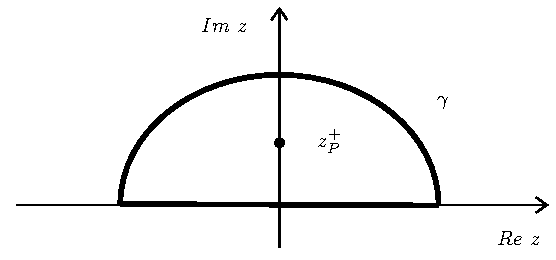
\includegraphics[width=0.6\textwidth]{../lessons/18_image/1.pdf}
\caption{\label{fig:18_1} Positive integration contour \( \gamma   \) in the complex plane for the integral \( I \). It contains only the pole at \( +i \xi ^{-1} \).}
\end{figure}


Therefore, we have seen that for the Ising model \( \nu = 1/2 \). If we also consider the values of the other critical exponents we see that the upper critical dimension for this model is \( d=4 \). In other words, mean field theories are actually good approximations for the Ising model if \( d \geq 4 \). We will later see some other confirmations of this fact.





\section{Including fluctuations at the Gaussian level (non interacting fields)}
Until now even if we have introduced Ginzburg-Landau theory we are still neglecting the effects of the fluctuations since we are regarding the mean field theory approximation for non-homogeneous systems as a saddle point approximation of a more general theory; in other words, since we are approximating
\begin{equation*}
  Z_{GL} [h] \overset{\substack{ \text{saddle} \\  \text{point} } }{\simeq } Z_{GL}^0 [h] = e^{- L [m_0 (\va{r})]}
\end{equation*}
we are still regarding the magnetization \( m \) as non fluctuating over the system. In order to include the fluctuations we must do more and go further the simple saddle point approximation. The simplest way we can include fluctuations in our description is expanding \( Z \) expressed as a functional integral around the stationary solution and keeping only quadratic terms; this means that we are considering fluctuations that follow a normal distribution around the stationary value. The important thing to note, however, is that in this approximation these fluctuations are independent, i.e. they do not interact with each other. As we will see, with this assumption the values of some critical exponents will differ from the "usual" ones predicted by mean field theories.

Hence, let us introduce fluctuations at the Gaussian level. Consider consider \( h=0 \) and \( m_0 (\va{r})= m_0 \) be the solution of the saddle point approximation. Let us expand the general expression
\begin{equation*}
  \beta \mathcal{H}_{eff}  [m (\va{r})] = \int_{}^{}  \qty( a t m^2 + \frac{b}{2} m^4 + \frac{k}{2} \qty(\va{\grad } m)^2 ) \dd[d]{\va{r}}
\end{equation*}
by using
\begin{equation*}
  m(\va{r}) = m_0 + \delta m(\va{r})
\end{equation*}
If we assumed that the fluctuations \(  \delta m(\va{r})\) are small, we would obtain:
\begin{subequations}
\begin{align*}
   \qty(\grad m)^2 &= \qty(\grad \qty(m_0 + \delta m) )^2 = \qty(\grad \qty(\delta m) )^2  \\
     m^2 &= m_0^2 + 2 m_0 \delta m + \qty(\delta m)^2 \\
     m^4 &= m_0^4 + 4 m_0^3 \delta m + 6 m_0^2 (\delta m)^2 + 4 m_0 \delta m^3 + (\delta m)^4
\end{align*}
\end{subequations}
Hence, we have
\begin{equation}
  \beta \mathcal{H}_{eff} = V \underbrace{ \qty(a t m_0^2 + \frac{b}{2} m_0^4) }_{A_0}
  + \int_{}^{} \qty(\frac{k}{2}\qty( \va{\grad } (\delta m))^2 + \qty(a t + 3 b m_0^2)\delta  m^2 + 2 b m_0 \delta m^3 + \frac{b}{2} \delta m^4 )\dd[d]{\va{r}}
\end{equation}
where \( V \) is the volume of the system and the term proportional to \( \delta m \),  \( \qty( 2 a t m_0  +  2b m_0^3 )  \), is zero since \( m_0 \) is the solution of the extremal condition (\( m_0 \) is the stationary solution)
\begin{equation*}
  \eval{\frac{\delta \mathcal{H}_{eff}}{\delta m}}_{m=m_0} = 0
\end{equation*}
For simplicity let us first consider \( T>T_c \); in this case, we know that \( m_0 = 0 \) and hence,
\begin{equation*}
   m (\va{r}) = m_0 + \delta m(\va{r}) = \delta m (\va{r})
\end{equation*}
We have also \( A_0 =0 \),  \( 3bm_0^2 \delta m^2 = 0 \) and \( 2 b m_0 \delta m^3 = 0 \). Taking all of this into account, we obtain:
\begin{equation*}
  \beta \mathcal{H}_{eff}^{T>T_c} (\delta m)= \int_{}^{} \dd[d]{\va{r}} \qty(\frac{k}{2} \qty(\va{\grad }\delta m)^2 + a t (\delta m)^2 + \frac{b}{2} (\delta m)^4 )
\end{equation*}
The Gaussian approximation consists in neglecting the quartic term \( (\delta m)^4 \), hence we finally obtain:
\begin{equation}
    \beta \mathcal{H}_{eff}^{T>T_c} (\delta m) \simeq  \int_{}^{} \dd[d]{\va{r}} \qty(\frac{k}{2} \qty( \va{\grad } \delta m)^2 + a t (\delta m)^2 )
\end{equation}
\begin{remark}
It is important to understand that these are fluctuations with respect to the solution \( m_0 \).
\end{remark}








\section{Ginzburg-Landau in the Gaussian approximation}

Let us solve
\begin{equation}
  Z_{GL}^G = \int_{}^{} \text{D} \qty[\delta m] e^{- \int_{}^{} \dd[D]{r} \qty(\frac{k}{2} \qty(\grad \delta m)^2 + a t (\delta m)^2  )  }
 \end{equation}
 in the Fourier space.  Consider a system in a box of volume \( V = L^D \) (periodic boundary conditions):
 \begin{equation}
   \delta m (\va{r}) = \frac{1}{V} \sum_{\va{k}}  e^{i \va{k}\vdot \va{r}} (\delta m_{\va{k}})
 \end{equation}
where
\begin{equation}
  \delta m_{\va{k}} = \int_{V}^{}  \delta m (\va{r}) e^{-i \va{k} \vdot \va{r} }\dd[D]{\va{r}}
\end{equation}
where \( \va{k} = k_1, \dots, k_D = \frac{2 \pi  \bar{n} }{L}\) with \( k_ \alpha = \frac{2 \pi }{L} n_ \alpha  \) \( (n_ \alpha  = 0 , \pm 1, \dots) \).
\begin{remark}
  We have \( \delta m_{\va{k}} \in \mathbb{C} \) but \( \delta m (\va{r}) \in \R \), hence
  \begin{equation}
    \delta m_{\va{k}} = - \delta m^*_{-\va{k}}
  \end{equation}
\end{remark}

\subsection{Useful relations}
Sometimes it is useful to convert the sum over \( \va{k} \) by an integral by using the density of states in the \( \va{k} \) space that is \( \frac{V}{(2 \pi )^D} \),
\begin{empheq}[box=\myyellowbox]{equation}
  \sum_{\va{k}}^{} \rightarrow \frac{V}{( 2 \pi )^D} \int_{\R^D}^{} \dd[]{\va{k}}
\end{empheq}
Hence,
\begin{equation}
\begin{split}
  \frac{1}{V} \sum_{\va{k}}^{} e^{i \va{k} (\va{r}-\va{r}')} & \rightarrow \frac{1}{V} \frac{V}{(2 \pi )^2} \int_{\R^D}^{} \dd[D]{\va{k}} e^{i \va{k} (\va{r}-\va{r}')} \\
  & = \frac{1}{(2 \pi )^D} \int_{\R^D}^{} e^{i \va{k} (\va{r}-\va{r}')} \dd[D]{\va{k}}  = \delta (\va{r}- \va{r}')
\end{split}
\end{equation}
so
\begin{empheq}[box=\myyellowbox]{equation}
  \frac{1}{V} \sum_{\va{k}}^{} e^{i \va{k} (\va{r}-\va{r}')} \rightarrow \delta (\va{r}-\va{r}')
\end{empheq}
Inserting
\begin{equation}
  m (\va{r}) = \frac{1}{V} \sum_{\va{k}}^{} e^{i \va{k}' \va{r}} m_{\va{k}'}
\end{equation}
In the expression
\begin{equation}
  m_{\va{k}} = \int_{V}^{} \dd[D]{\va{r}} e^{- i \va{k} \vdot \va{r}} m (\va{r})
 \end{equation}
one gets
\begin{empheq}[box=\myyellowbox]{equation}
  \frac{1}{V} \int_{}^{} \dd[D]{\va{r}} e^{i (\va{k} - \va{k}') \vdot  \va{r}} = \delta _{\va{k}\va{k}'}
  \label{eq:18_1}
\end{empheq}
Finally, since
\begin{equation}
  \int_{}^{} \dd[D]{\va{r}} e^{i (\va{k}-\va{k}') \vdot \va{r}} \overset{V \rightarrow \infty }{\longrightarrow  } (2 \pi )^D \delta (\va{k}-\va{k}')
\end{equation}
From \eqref{eq:18_1} one gets,
\begin{empheq}[box=\myyellowbox]{equation}
  V \delta _{\va{k} \va{k}'} \overset{V \rightarrow \infty }{\longrightarrow  } (2 \pi )^D \delta (\va{k} - \va{k}')
\end{empheq}
\begin{remark}
Since the minimal spatial length of the system is \( a \),
\begin{equation}
  a \Rightarrow \abs{\va{k}} \le \frac{\pi }{a} = \Lambda
\end{equation}
that is the ultraviolet cut-off.
\end{remark}


\section{Gaussian Hamiltonian in Fourier space}
For simplicity, let us change notation
\begin{equation}
  \delta m (\va{r}) \leftrightarrow \varphi (\va{r}), \quad k \leftrightarrow c
\end{equation}
obtaining
\begin{equation}
  \beta \mathcal{H}_{eff}^{G,>} [\varphi ]= \int_{}^{} \dd[D]{\va{r}} \qty[\frac{c}{2} \qty(\grad \varphi )^2 + a t \varphi  ^2 ]
  \label{eq:18_2}
\end{equation}
where
\begin{equation}
  \varphi (\va{r}) = \frac{1}{V} \sum_{\va{k}}^{} e^{i \va{k} \vdot \va{r}} \varphi _{\va{k}}
\end{equation}
Consider the term of expression \eqref{eq:18_2} separately:
\begin{itemize}
\item Term \( a t \varphi ^2 \).
\begin{equation}
  \int_{}^{} \dd[D]{\va{r}} a t \varphi ^2 (\va{r}) = \frac{a t}{V^2} \sum_{\va{k},\va{k}'}^{}  \int_{\R^D}^{} e^{i (\va{k}+\va{k}') \vdot \va{r}} \varphi _{\va{k}} \varphi _{\va{k}'} \dd[D]{\va{r}}
  = \frac{at}{V^2} \sum_{\va{k}\va{k}'}^{} \varphi _{\va{k}} \varphi _{\va{k}'} \delta (\va{k}+\va{k}') (2 \pi )^D
\end{equation}
On the other hand,
\begin{equation}
  \frac{(2 \pi )^D}{V} \delta (\va{k}+ \va{k}') \overset{V \gg 1}{\longrightarrow} \delta _{\va{k},-\va{k}'}
\end{equation}
\begin{equation}
  \Rightarrow \int_{}^{} \dd[D]{\va{r}} a t \varphi ^2 (\va{r})  \overset{V \gg 1}{\longrightarrow} \frac{1}{2V} \sum_{\va{k}}^{} 2 a t  \varphi _{\va{k}} \varphi _{\va{k}'}
\end{equation}
\item Term \( \int_{}^{} \dd[D]{\va{r}} \frac{c}{2} \qty(\grad \varphi )^2    \).
\begin{equation}
\begin{split}
  \int_{}^{} \dd[D]{r} \frac{c}{2} \qty(\grad \varphi )^2 & = \frac{c}{2} \frac{1}{V^2} \int_{}^{} \dd[D]{\va{r}} \qty(\grad \sum_{\va{k}}^{} e^{i \va{k} \vdot \va{r}} \varphi _{\va{k}}  ) \qty(\grad \sum_{\va{k}'}^{} e^{i \va{k}' \vdot \va{r} } \varphi _{\va{k}'}  )     \\
  & = \frac{c}{2 V^2} \sum_{\va{k} \va{k}'}^{}  \qty(- \va{k} \vdot \va{k}') \varphi _{\va{k}} \varphi _{\va{k}'} \underbrace{\int_{}^{} \dd[D]{\va{r}}  e^{i (\va{k}+\va{k}')\vdot \va{r}}}_{(2 \pi )^2 \delta (\va{k}+ \va{k}') \rightarrow V \delta _{\va{k},-\va{k}'}}   \\
  & = \frac{c}{2V} \sum_{\va{k}}^{} \abs{\va{k}}^2 \varphi _{\va{k}} \varphi _{\va{-k}'}
\end{split}
\end{equation}
\end{itemize}
In summary, the exponent is:
\begin{empheq}[box=\myyellowbox]{equation}
  \beta \mathcal{H}_{eff}^{G,>} \rightarrow \frac{1}{2V} \sum_{\va{k}}^{} \qty(2 a t + c k^2) \varphi _{\va{k}} \varphi _{-\va{k}'}
\end{empheq}
this is the Gaussian model in Fourier space.

Now, the question is: how can we write the measure \( \int \text{D}[\varphi ] \) in Fourier space?
\begin{equation}
  \varphi (\va{r}) = \frac{1}{V} \sum_{\va{k}}^{} \varphi _{\va{k}} e^{i \va{k} \vdot \va{r}}, \quad \varphi _{\va{k}} \in \mathbb{C}
\end{equation}
\begin{equation}
  \int_{}^{} \text{D} \qty[\varphi (\va{r})] \rightarrow \int_{- \infty }^{+ \infty } \prod_{\abs{\va{k}} < \Lambda  }^{}   \dd[]{(\Re{\varphi _{\va{k}}})}   \dd[]{(\Im{\varphi _{\va{k}}})}
\end{equation}
with \( \varphi (\va{r}) \in \R \), that implies \(    \varphi _{\va{k}}^* = \varphi _{-\va{k}}\), hence
\begin{equation}
  \begin{cases}
   \Re {\varphi _{\va{k}}} = \Re {\varphi _{-\va{k}}} \\
  \Im{\varphi _{\va{k}}} = -\Im {\varphi _{-\va{k}}}
  \end{cases}
\end{equation}
Therefore, if we considered
\begin{equation}
  \prod_{\abs{\va{k}} < \Lambda  }^{} \dd[]{\Re {\varphi _{\va{k}}}} \dd[]{\Im{\varphi _{\va{k}}}}
\end{equation}
we would count twice. We need to consider one restriction. For example we can assume
\( k_z > 0 \) (hupper half of the \( \va{k} \) space), hence
\begin{equation}
  \Tr \equiv \int_{- \infty }^{+ \infty } \prod_{\substack{ \abs{\va{k}} < \Lambda   \\ k_z > 0 } }^{}   \dd[]{\Re {\varphi _{\va{k}}}}  \dd[]{\Im {\varphi _{\va{k}}}}
\end{equation}
or
\begin{equation}
  \Tr \equiv \frac{1}{2} \int_{- \infty }^{+ \infty } \prod_{\substack{ \abs{\va{k}} < \Lambda    } }^{}   \dd[]{\Re {\varphi _{\va{k}}}}  \dd[]{\Im {\varphi _{\va{k}}}}
\end{equation}
For sake of brevity
\begin{equation}
  \Tr \equiv \int_{-\infty }^{+\infty } \prod_{\va{k}}^{'}  \dd[]{\varphi _{\va{k}}}
\end{equation}
where
\begin{equation}
  \prod_{\va{k}}^{} \dd[]{\varphi _{\va{k}}} \equiv \prod_{\substack{ \abs{\va{k}} < \Lambda   \\ k_z >0 } }^{}   \dd[]{\Re {\varphi _{\va{k}}}}  \dd[]{\Im {\varphi _{\va{k}}}}
\end{equation}
In summary, we have
\begin{equation}
  \widetilde{Z}_{GC}^{G,>} =  \int_{- \infty }^{+ \infty }  \qty( \prod_{\va{k}}^{'}  \dd[]{\varphi _{\va{k}}})
  e^{- \beta \widetilde{\mathcal{H}}_{eff}^G [\varphi _{\va{k}}] }
\end{equation}
where
\begin{equation}
  - \beta \widetilde{\mathcal{H}}_{eff}^G [\varphi _{\va{k}}] = - \frac{1}{2V} \sum_{\va{k}}^{} \qty(2at+c \abs{\va{k}}^2 ) \abs{\varphi _{\va{k}}}^2
\end{equation}
\subsection{Free energy in Gaussian approximation}
Let us consider the case \( T>T_c \) \( (m_0=0) \) and \( h=0 \)
\begin{equation}
  \widetilde{Z}_G^{T>T_c} = \prod_{\va{k}}^{'} \int_{-\infty }^{+\infty } \dd[]{\Re {\varphi _{\va{k}}}}  \dd[]{\Im {\varphi _{\va{k}}}} e^{- \frac{1}{2V} \sum_{\va{k}}^{} \qty(2at+c \abs{\va{k}}^2 ) \abs{\varphi _{\va{k}}}^2}
\end{equation}
Change variables
\begin{equation}
  \begin{cases}
   x \equiv  \Re \varphi _{\va{k}}\\
  y \equiv  \Im \varphi _{\va{k}}
  \end{cases}
\end{equation}
and since
\begin{equation}
  \int_{-\infty }^{+\infty } \dd[]{x} \dd[]{y} e^{-A (x^2+y^2)} = \frac{\pi }{A}
\end{equation}
with \( A \equiv  \frac{1}{2V} \).
\begin{equation}
  e^{-\beta \widetilde{F}_{GL}^> } = \qty(\prod_{\substack{\va{k} \\ \abs{\va{k}} <\Lambda \\ k_z > 0  } }^{'}  \frac{2 \pi V}{2 a t + c \abs{\va{k}}^2 } )
  = \exp [\frac{1}{2} \sum_{\abs{\va{k}}<\Lambda  }^{} \log (\frac{2 \pi V}{2 a t + c \abs{\va{k}}^2 })   ]
\end{equation}
Hence,
\begin{equation}
  \widetilde{F}_{GL}^{G,T>T_c} = - \frac{1}{2} k_B T \sum_{\abs{\va{k}}< \Lambda  }^{}
  \log{\qty(\frac{2 \pi V}{2 a t + c \abs{\va{k}}^2 })}
\end{equation}
\begin{remark}
For \( T<T_c \) we have \( m_0 \neq 0 \). In addition, to redefine the quadratic term \( (at+3bm_0^2) \), that for \( m_0^2 = - at/b \), becames \( -2at \) we have also the term
\begin{equation}
  V A_0 = V (atm_0^2 + \frac{b}{2} m_0^4)
\end{equation}
Therefore,
\begin{equation}
  \widetilde{F}_{GL}^{G,T<T_c} = \beta A_0 V - \frac{1}{2} k_B T \sum_{\abs{\va{k}}< \Lambda  }^{}
  \log{\qty(\frac{2 \pi V}{2 a t + c \abs{\va{k}}^2 })}
\end{equation}
\end{remark}

\subsection{Specific heat in the Gaussian approximation}
\begin{equation}
  c_V^G = - T \pdv[2]{F^G/V}{T} \overset{to do}{=}   \underbrace{\frac{A}{V} \sum_{\abs{\va{k}} < \Lambda  }^{}
  \frac{1}{ \qty(2 a t + c \abs{\va{k}}^2 )^2}}_{1^{st}}
    - \underbrace{ \frac{B}{V} \sum_{\abs{\va{k}}< \Lambda  }^{} \frac{1}{2 a t + c \abs{\va{k}}^2 }}_{2^{st}}
\end{equation}
One can show that
\begin{equation}
1^{st} \propto
  \begin{cases}
   \xi ^{4-D} \sim t^{-\nu (4-D)}  & D < 4\\
  < \infty & D > 4
  \end{cases}
\end{equation}
\begin{equation}
2^{nd} \propto
  \begin{cases}
   \xi ^{2-D} \sim t^{-\nu (2-D)}  & D < 2\\
  < \infty & D > 2
  \end{cases}
\end{equation}
In summary, the behaviour of the specific heat is
\begin{equation}
  c_V \sim \begin{cases}
    t^{-\nu (4-D)} & D < 4 \\
    <\infty & D > 4
\end{cases}
\end{equation}
The introduction of the fluctuations even if only at the Gaussian level changes the behaviour of \( c_V \) at the transition point.

\begin{figure}[h!]
\begin{minipage}[c]{0.5\linewidth}
\subfloat[][Description]{ 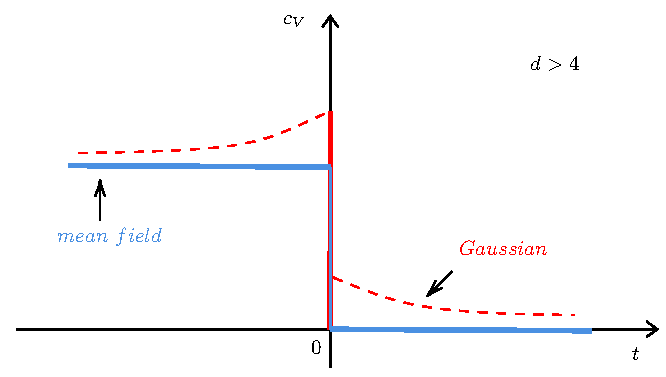
\includegraphics[width=1\textwidth]{../lessons/18_image/2.pdf}  \label{fig:18_2_1} }
\end{minipage}
\begin{minipage}[]{0.5\linewidth}
\centering
\subfloat[][Description]{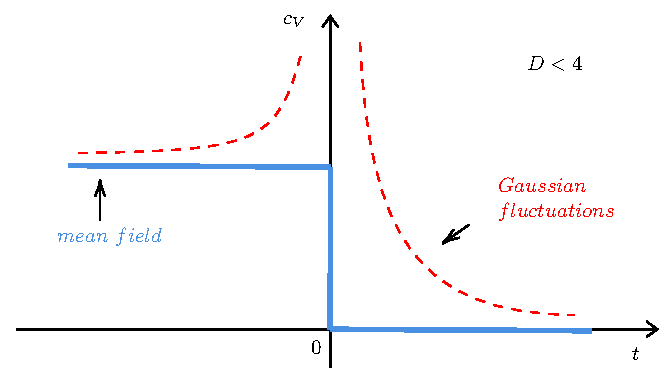
\includegraphics[width=1\textwidth]{../lessons/18_image/3.pdf}  \label{fig:18_2_2} }
\end{minipage}
\caption{\label{fig:} }
\end{figure}

The introduction of Gaussian fluctuations gives rise to a divergence in \( c_V \sim t^{- \alpha } \) with
\begin{equation}
  \alpha = \nu (4-D) \quad \text{for } D < 4
\end{equation}

\subsection{How about \( \nu  \)?}
We have to compute the \( 2- \)point correlation function for \( \mathcal{H}_{eff}^G (\varphi ) \) that in Fourier space become
\begin{equation}
  \expval{\varphi _{\va{k}} \varphi _{\va{k}'}}_G =
\frac{\int_{- \infty }^{+ \infty } \dd[]{ \tilde{ \varphi} _{\va{k}_1} }  \dots
  \dd[]{ \tilde{ \varphi} _{\va{k}} }  \dd[]{ \tilde{ \varphi} _{\va{k}'} }
 \tilde{\varphi} _{\va{k}} \tilde{\varphi} _{\va{k}'} \dots
  e^{- \beta \mathcal{H}_{eff}^G}  \dots
 }{
 \int_{- \infty }^{+ \infty } \dd[]{ \tilde{ \varphi} _{\va{k}_1} }  \dots
   \dd[]{ \tilde{ \varphi} _{\va{k}} }  \dd[]{ \tilde{ \varphi} _{\va{k}'} } \dots
   \dd[]{ \tilde{ \varphi} _{\va{k}_n} } \dots
 }
\end{equation}
where
\begin{equation}
  \mathcal{H}_{eff}^G = A_0 V + \frac{1}{2V} \sum_{\va{k}}^{} \qty(2 a t + c \va{k}^2) \abs{\varphi _{\va{k}}}^2
\end{equation}
It is possible to show:
\begin{equation}
  \expval{\varphi _{\va{k}} \varphi _{\va{k}'}}_G = \delta _{\va{k},-\va{k}'} \frac{V}{2 a t + c k^2}
\end{equation}
that, in the limit \( V \rightarrow \infty  \) becomes
\begin{equation}
    \expval{\varphi _{\va{k}} \varphi _{\va{k}'}}_G \overset{V \rightarrow \infty }{\longrightarrow} \frac{(2 \pi )^D}{2 a t + c \va{k}^2} \delta ^D (\va{k}+ \va{k}')
\end{equation}
By antitrasforming
\begin{equation}
\begin{split}
  \expval{\varphi (\va{r}) \varphi (\va{r}')}_G &= \frac{1}{V^2} \sum_{\va{k}, \va{k}'}^{} e^{i (\va{k}\vdot \va{r} + \va{k}' \vdot \va{r}' )} \expval{\varphi _{\va{k}} \varphi _{\va{k}'}}_G    \\
  & = \frac{1}{V^2} \sum_{\va{k}, \va{k}'}^{} e^{i (\va{k}\vdot \va{r} + \va{k}' \vdot \va{r}' )}  \delta _{\va{k}, -\va{k}'} \frac{V}{2at+ck^2} \\
  & = \frac{1}{V} \sum_{\va{k}}^{} \frac{ e^{i \va{k}\vdot ( \va{r} - \va{r}' )}}{2 a t + c k^2}
\end{split}
\end{equation}
Using
\begin{equation}
  \xi _> (t) = \qty(\frac{c}{2at})^{1/2}
\end{equation}
we get
\begin{equation}
    \expval{\varphi (\va{r}) \varphi (\va{r}')}_G = \frac{1}{V_c} \sum_{\va{k}}^{} \frac{ e^{i \va{k}\vdot ( \va{r} - \va{r}' )} }{k^2 + \xi _>^{-2}}
    = \frac{1}{V} \sum_{\va{k}}^{} e^{i \va{k} \vdot \va{x}} \hat{G} (\va{k})
\end{equation}
where
\begin{equation}
  \hat{G} (\va{k}) = \frac{1}{c \qty(k^2 + \xi _>^{-2}) }
\end{equation}
i.e. is of the same form found in mean field.
\begin{equation}
\Rightarrow
  \begin{cases}
   \nu _G = \frac{1}{2}\\
   \eta_G = 0
  \end{cases}
\end{equation}
There are no changes with Gaussian fluctuation! Interactions between \( \varphi _{\va{k}} \) are needed!






\end{document}
